%%%%%%%%%%%%% Final Project Documentation %%%%%%%%%%%%%%%%%%
\documentclass[a4paper,10pt]{article}

\usepackage[backend=biber]{biblatex}
\usepackage{float} 
\usepackage{wrapfig}
\usepackage[skins]{tcolorbox}
% \usepackage{fontenc}
\usepackage{geometry} 
\usepackage[font=small,labelfont=bf]{caption}
\usepackage{blindtext} 
% \usepackage{textcomp}
\usepackage[hidelinks]{hyperref}
\usepackage{lipsum}
\usepackage{bm} 
\usepackage{listings}
\usepackage{amsmath}  
\usepackage{color}    
\usepackage{framed} 
\usepackage{changepage}
\usepackage{tikz,pgfplots}
\usepackage{graphicx}
\usepackage{lmodern}

\addbibresource{citations.bib}
 
\DeclareLabeldate{\field{date}\field{eventdate} \field{origdate}\literal{nodate}}

\linespread{1.05} % Line spacing

\pgfplotsset{every axis/.append style={thick},width=10cm,height=4cm,compat=1.9}

\definecolor{mygreen}{rgb}{0,0.6,0}
\definecolor{mygray}{rgb}{0.5,0.5,0.5}
\definecolor{mymauve}{rgb}{0.59,0,0.92}
\definecolor{mysoftgrey}{rgb}{0.95,0.94,0.94}

% Creates a nice place to put code 
\lstnewenvironment{codebox}[1][] {
	\noindent
	\minipage{\linewidth}
		\medskip  
		\lstset{ 
			backgroundcolor=\color{mysoftgrey},
			basicstyle=\footnotesize\ttfamily,
			breakatwhitespace=false,         
			breaklines=true,                 
			commentstyle=\color{mygreen},    
			deletekeywords={...},            
			escapeinside={\%*}{*)},          
			extendedchars=true,              
			frame=single,                    
			keepspaces=true,                 
			keywordstyle=\color{blue},       
			language=C++,                    
			otherkeywords={*,...,a,b,ary_},  
			numbers=left,                    
			numbersep=5pt,                   
			numberstyle=\tiny\color{mygray}, 
			rulecolor=\color{black},         
			showspaces=false,                
			showstringspaces=false,          
			showtabs=false,                  
			stepnumber=1,                    
			stringstyle=b,                   
			tabsize=4,                       
			title=\lstname                   
		}
	}   
	{\endminipage}
 
% \renewcommand*\rmdefault{cmr}

\let\oldemph\emph
\renewcommand{\emph}[1]{\textbf{\oldemph{#1}}}

\let\oldurl\url 
\renewcommand{\url}[1]{ { \footnotesize{\oldurl{#1}} } }

\newcommand{\mathwords}[1]{
	{
		\linespread{.95}
		\begin{adjustwidth}{8em}{8em}
			\footnotesize
			#1 
		\end{adjustwidth}
	}
}

\newenvironment{funfact}[2][r]{
	\par
	\wrapfigure{#1}{0.5\textwidth}
		\begin{minipage}{0.48\textwidth}
			\vspace{-1em}
			\begin{tcolorbox}[
					left=1mm,
					right=1mm,
					top=.5mm,
					bottom=.5mm,
					boxsep=1mm,
					title=#2,
					fonttitle=\sffamily,
					colback=black!2!white,
					colbacktitle=black!75!,
					colframe=black!100!black,
					arc=0pt,
					outer arc=0pt ]
				\linespread{.95}
				\small
}
{
			\end{tcolorbox}
			\vspace{-1em}
		\end{minipage}	
	\endwrapfigure
}

\newcommand{\code}[1]{ {\fontfamily{lmtt}\fontseries{b}\selectfont
	#1}
}

\setlength{\parindent}{2em}
\setlength{\parskip}{0.7em}


\begin{document}


% ----------------------------------------------------------------------------------------

\pagenumbering{Alph} 
\begin{titlepage}

\newcommand{\HRule}{\rule{\linewidth}{0.5mm}} % Defines a new command for the horizontal lines, changes thickness

\center

\textsc{\LARGE University of Utah}\\[1.5cm]
\textsc{\Large Introduction to Computational Physics }\\[0.5cm]
\textsc{\large Spring 2015}\\[0.5cm]

\HRule \\[0.4cm]
{ \huge \bfseries Neural Net Architecture}\\[0.4cm]
{ \huge \bfseries With Demo Application}\\[0.1cm]
\HRule \\[1.cm]

\begin{minipage}{\textwidth}
\begin{flushleft} \large
\emph{Author:}\\  
Derek \textsc{Strasters}
\end{flushleft}
\end{minipage}
\\[3cm]

{\large \today}\\[4.0cm]


\includegraphics[scale=00.55]{images/Logo.png}\\

\vfill

\end{titlepage} 
\pagenumbering{arabic}

%----------------------------------------------------------------------------------------%
%	TABLE OF CONTENTS                                                                    %
%----------------------------------------------------------------------------------------%

\large\tableofcontents
\newpage\normalsize

%----------------------------------------------------------------------------------------%
%	INTRODUCTION / Section 1                                                             %
%----------------------------------------------------------------------------------------%
 


\section{Introduction to this Neural Network Architecture}

\subsection{Preface}

The Neural Net Architecture being presented here is built with the intention of providing another programmer with a
broad set of tools for the creation of a Neural Net. To make this demonstration complete, there is within the project
directory a source file named \texttt{Alan.cpp} (honouring one of the fathers of computer science, Alan Turing).
Alan, compiles compiles into an executable interactive demonstration that is meant to offer somewhat of a visual
observation on the inner workings of a neural network.  The demonstration shows just one of the most simple examples of
the many exciting ways in which a user might make use of an architecture such as this to implement a Neural Network.
It is my hope to continue to improve the user-friendliness, efficiency, and open-endedness with such goals as
implementing the OpenGL library to make use of the powerful video cards in most home computers, and full cross platform
windowed user interface. There truly are innumerable possibilities for the uses of neural networks, and I think it would
be just neat if we could make them as readily available to the world as perhaps an on-line calculator is now. This has
been the main driving factor behind my attempt at a design that both leaves room for users to easily make modifications
in places that are likely to be experimented with, while also maintaining a reasonably small number of easy to use
classes and functions to handle the heavy computing that are designed with the intent to make it difficult for the user
to introduce bugs by accident.

\subsection{An Abstract Definition}

Before continuing, a brief explanation of what a neural net actually is, is in order.  My own source of understanding
Neural Networks has come from a web book by Michael Nielsen whom I recommend to any
interested readers interested in more information about neural networks \cite{NetWeb}. An interesting side point
about his book, is that it's not even finished, he's publishing it as he goes.

A neural network or, neural net, is so named because of it's (somewhat crude) semblance to the manner in which a brain's
network of neurons work.  It is not, however, identical by any means.  In the shortest way of stating a neural nets
function, it is a system that is capable of ``learning'' how to behave.  For example, in the demo implementation, a
network is constructed and then ``shown'' some information.  At the same time, the network is also ``shown'' what
outcome we want it to produce, and after we do this many times, we stop the so called training and can then present the 
network a value it has never seen and hopefully it will have learned to respond in the way we have taught it.

Now this may sound at the surface like a really inefficient way of doing nothing more complicated than regurgitating
values from some kind of look up table of recorded values.  The thing that makes this type of system so much more
special than trivial behaviour of a look up table is that you can then show the network some data it has never been
exposed to before and if that data follows some pattern, even a pattern that we ourselves are unaware of, it is very
likely going to output the correct response to that new data.  It's a matter of interpretation, but this student finds
such behavior to be moving the idea of a computer that could arguably said to ``think'' is arriving in a much
\emph{less} distant future.

\subsection{Backpropagation by Stochastic Gradient Descent}

I will go into greater detail on the specifics of my design later, but for now the idea behind a neural net is
that a set of items, call them neurons, are linked together in a network in the sense that a neuron may read data
from other neurons that it is linked to. These neurons have the capability of reading in multiple numerical values
(typically values between 0 and 1) as impetus for generating a singular output value. For now I will just say that the
neuron simply does \emph{something} with those values to generate it's output. It is unsurprising that most of the
neurons will be taking the outputs of other many other neurons as input. Knowing nothing more than what has been stated
- \textit{\ldots a semblance to the manner in which a brain's network of neurons work,} - and that each neuron accepts
the ouputs from many other neurons, it then seems reasonable to expect that each neuron has a way in which to grant
greater weight to some inputs and less weight to others. The way in which this concept is implemented in this type of
Neural Network is for each neuron to keep a simple scalar for each of it's inputs.  These scalars are aptly called the
neuron's \textmd{weights}.  To use the brain analogy, the neuron's \textbf{weights} strengthen or weaken the synapses
between other neurons.  This implies the need for some feedback mechanism capable of modifying the weights to
produce the desired behavior of the network. Adding to the idea of weights, each neuron also keeps a singular value that
acts as a scalar to it's output; this is called the \textbf{bias} and must also subject to change by our feedback
mechanism.  We will soon see that it is useful to define an equation for the sum of weighted inputs to which the bias is
added, a value that is often represented as $Z$.

\begin{equation}\label{Zval} 
Z \equiv \left( \sum^N_{j=0} w_j a_j \right)   + b
\end{equation}

\mathwords{ Where $w$ is a weight, $a_j$ is an input values, $N$ the total number of inputs, and $b$ the bias.} 

This looks like it could be that \emph{something} I had referred to earlier that the neurons are doing with their input
data, but in our case, it is not -- although it is part of it.  To elicit Boolean logic type behavior (not to say that
this is the best behavior we could want), we should desired that we have an output that behaves somewhat like a switch,
since that is what is going to dive any logic type computations that develop in the network but,  as we will see, we
also want a smooth function that describes our output.  This comes back to our feedback mechanism for changing the
weights and biases of the system, a method called \emph{Backpropagation}.

\subsubsection{The Sigmoid Neuron}

\setlength{\parskip}{0em} % Should this be a wrapper environment?
Before discussing Backpropagation we will need to look at the underlying concept of \textbf{Gradient Descent}.  As one
can imagine with any appreciable amount of neurons in a network we are going to have a very large amount of variables
that will need to be ``tuned" through a training algorithm to make our system behave as desired.  For a network of the
type discussed here containing 9 neurons there could be up to 36 such variables, and a network of 25 could have up to
150.  Remember, what we are looking for is a best value for how well the system is producing expected results, a measure
we shall now define as \textbf{cost}. To optimize cost over such a large set of variables one might first think to use
a evolutionary or genetic algorithm, which wouldn't be a bad place to start, but a more direct route would certainly be
desirable in terms of the time it takes to find an optimal solution.  The more efficient strategy used in our system is
best described as treating each variable as a dimension, in the same sense that we move about in our 3 dimensions.
An algorithm then estimates the gradient of the cost over these dimensions with the values thereof pointing to a local
or hopefully global minima.  
\begin{funfact}{On Perceptrons}
In the earliest neural networks, equation \ref{Zval} was used to determine a binary neuron output by the simple rule:

\begin{align*}
	a = \left\{
  		\begin{array}{lr} 
    		a = 0 & : Z <   0 \\
    		a = 1 & : Z \ge 1
  		\end{array}
	\right.
\end{align*} 

Neurons of this type are called Perceptrons. They were a revolutionary idea developed by Frank
Rosenblatt \cite{WikiFrankRosenblatt} in 1957. There are however limitations in Perceptrons' ability to learn, a point
which newer systems seek to address with the methods found within this text.

\end{funfact}  
\noindent
To liken this to our 3 dimensional reality again, it would be as though one were standing
on a mountain, altitude being a measure of cost in this case, and looking at the slope of the ground near your feet to determine how to
get to the bottom of the mountain.  I rather like this analogy because it elucidates a similar pitfall experienced by
the neural network, if our mountain climber judges the slope by looking too near his feet, he may find himself eventually
stuck in a ditch or crevasse before reaching bottom.  If he judges the slope by looking too far into the distance, he
may end up traveling from mountain to mountain aimlessly never realizing if he were for a moment in the lowest spot. 
Enough about mountain men though, we should finish defining the behaviour of the neurons of this system.  The reason
Gradient Descent is important to how our neurons work is that if we were to use a step function (See \textbf{On Perceptrons})
there would be no mountains, only cliffs.  We need a function that is smooth such that we can calculate a gradient
therefrom.  Our neurons implement what is called an \emph{activation} function to do this, and there are many different
types, but they more or less have the same features -- they are continuous, smooth, and they act Boolean-like at their
extremities. What I mean by that is that it is desired that our neurons have an output that behaves somewhat like a
switch, since that is what is going to help logic type computations that develop in the network.  The activation
function we apply what is called the \textbf{Sigmoid} function $\boldsymbol\sigma$.  This function is applied directly
to the $Z$ value as shown in the following definition:
\setlength{\parskip}{0.7em}

\begin{equation}\label{Sigmafunc}
\sigma(z) \equiv \frac{1}{1+e^{-z}} 
\end{equation} 

\mathwords{\centering Definition of the Sigmoid function.}



\begin{figure}[H]
\centering
	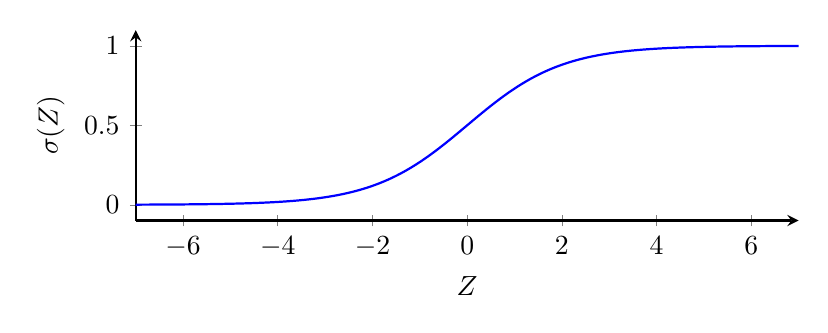
\begin{tikzpicture}
		\begin{axis}[
		    axis lines = left,
		    xlabel = $Z$,
		    ylabel = {$\sigma(Z)$},
		    enlarge y limits=auto
		]
		%Here the sigmoid is defined
		\addplot [
		    domain=-7:7, 
		    range=-0.05:0.05,
		    samples=1000, 
		    color=blue,
		    ]
		    {1 / (1 + exp(-x))};		 
		\end{axis}
	\end{tikzpicture}
	
	\caption{A plot of the Sigmoid function}
	\label{fig:SigPlot}
\end{figure}

\bigskip

START HERE
There is still the problem of figuring out by what
measure we want to determine how ``good'' are neurons are behaving and whether to strengthen or weaken their bonds. 
Well I'm going to jump ahead a little by just stating that I'm describing what is called the Cost Function of our
network and it doesn't actually have a hard Type.  What I mean by that is there are a number of ways of measuring how
``good'' the output of the system is when compared against training data. It is good for our purposes you use the
somewhat natural intuition of using the mean squared error of the output against the expected output.  It turns out to
be \textit{very} good for our puropses, because when we take the derivative (which we'll end up needing), we get a
simple difference calculate that is very easy to process.  

\begin{figure}[H] 
\centering
	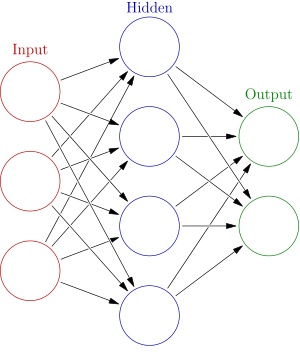
\includegraphics[width=0.5\textwidth]{images/network.png}
	\caption{Artificial neural network with layer coloring \protect\cite{NetImg}. \protect\footnotemark}
	\label{fig:NetImg}
\end{figure} 

\footnotetext{\fullcite{NetImg}}

So within our network the neurons are arranged into layers like what is shown in Figure \ref{fig:NetImg}.  You will
have data available to the so called input layer, each neuron takes the value in from every object that is in
front of it, if we take the front to be left. The values they take in could be either raw data or from other neurons of
course depending on where they're situated.  Now there are networks that will let neurons reach out other places
than just from the next layer, but the software I'm presenting as is stands now doesn't make that easy to do so I will
only be referring to the simple layer after layer variety.  Now we're setup to talk about the
cascade of events that is going to happen as our neurons do their action, which we now know to be finding $Z_i$ then
finding $\sigma(Z_i)$ .

So we place some data in front of the the input layer and tell the neurons to go ahead and look at it and start
calculate all the outputs or activations $a$, for the layer. The input layer reads the data and activated, the next
layer reads the input layer, and so on\ldots until reaching the output layer which we can then look at for the result. 
The first time through, as could be expected the data is more or less random, so now is when we've got our opportunity
to give the neurons some feed back that will determine how they should change their internal values.  Now comes the
second cascade of events that our neurons will perform, a concept known as back propagation.  Here the difference of the
expected outcome and the actual outcome if calculated, and using that to calculate the error $\delta$, the previous
layer will take $\delta$ and also each of the weights that were used against it and calculate it's error, and the
process repeats all the way back to the input layer.

To be more rigorous about what's happening, we shall be estimating the gradient of the \textbf{cost} function with
respect to $w$ and $b$ in terms of the expected outcome $y$, with the cost function being the aforementioned mean
squared error.  If we think of each layer as a vector, which has a matrix of weight values,
and another vector of bias values we can express the error of any given layer with:

\begin{equation}\label{errormatr}
\delta^l = ((w^{l+1})^T \delta^{l+1}) \odot \sigma'(z^l)
\end{equation}

{\centering\small Where $l$ is index of the current layer. 
\par}

We now have all the partial derivatives, here are the gradients for $w$ and $b$ 

\begin{gather}\label{gradientsw}
\nabla_w = \delta^{l+1}(a^l)^T\\
\nabla_b = \delta^{l+1}
\end{gather}

And then update your weights and biases negative of this multiplied by some constant.

\begin{gather}\label{graupdatw}
w^l \rightarrow
  w^l-\frac{\eta}{m} \sum_x \delta^{x,l} (a^{x,l-1})^T\\
b^l \rightarrow b^l-\frac{\eta}{m}
  \sum_x \delta^{x,l}
\end{gather}

Notice the $x$ in these equations. This representation assums that a mini-batch of items are selected at random from the
list of training data.  These equations show that we are taking the average of a mini-batch to update the \textbf{bias} and
\textbf{error} values of the system.
This process is the origin of the name stochastic backpropagation. Ok, lets move on to some actuall code now.

Within the Neural Net project directory there are a number of \textmd{c++} header and source files containing a number
of classes, structures, and functions many of which are \textmd{c++} templates.  These items will be briefly discussed
here.

There are also some sub-directories, the one named 'res' contains resources meant for use with the Neural Net
architecture to train on but this remains unimplemented at this time. The directory named 'DEMO' contains the files
needed to compile the working demo.

The reader may build and run the demo program by simply entering the 'DEMO' directory from a Linux terminal and entering
the command \texttt{make} followed by executing the now compiled file with the command\texttt{ ./DEMO}.
The reader may note that most of the header files do not have accompanying source files with the \texttt{.cpp} extent
ion; this is because most of the classes and functions of this architecture are templates for performance reasons.  The
template class member functions  and normal functions that are also templates are both declared and defined entirely in
the header file, this is because templates are evaluated at compile time based on their template parameters, the
compiler reserves memory for each unique set of template parameters. The only reason this is worth mentioning is because
it is a strategy for increasing performance in a sort of trade off between longer compile time and more memory usage is
exchange for faster execution. This also has the unfortunate effect that template parameters for things like an array
size cannot be declared at run time unless a compiler activity can be executed somewhere outside of the architecture's
files before any features of those classes are called upon (this is actually a planned feature for the future of this
project, I plan to be tinkering with and improving thiIs code for some time).

I will now enumerate the contents of each file, but I will only be listing \underline{some} of the more important
functions within due to the large number of functions that are defined.


%------------------------------------------------ 
%Neuron.h / Section 2                     
%------------------------------------------------ 

\section{Header File |\code{Neuron.h}} 

Within the header file of \code{Neuron.h} is a single class representing the most basic component of the Neural Net, the
\code{Neuron< >()}.

\subsection{Instantiable |\code{class Neuron< >()}}

This class contains all the field members that will be used extensively during operation of the Neural Net.  A
programmer will never need to interact directly with Neuron objects since any member access's or calls
made to  are handled by a friend class, the \code{Layer< >()} and other objects therefrom as we will see later.
Another point of interest is that no actual \code{Neuron< >()} objects will ever be instantiated.  This is
because \code{Neuron< >()} implements an \emph{abstract class} design patter, meaning that other
classes will extend this class as their parent class.  The derived, or child, classes will have all the member functions
and fields as \code{{Neuron< >()}} while still being able to have their own unique members, however what makes this class
\emph{abstract} is the interesting ability to call upon certain member functions of it's children classes,
regardless of what that child class is, so long as it has the functions with the correct name.  This is done using a
concept know as the \emph{Curiously Recurring Template Pattern} or just CRTP \cite{WikiCrtp} . Use of the CRTP opens up
all sorts of interesting possibilities, but our main use is for making calls to derived, children classes.

%------------------------------------------------
%GetActivationFct / Section 2
%------------------------------------------------

\subsubsection{Member Function |\code{FuncSig GetActivationFct()}}\label{activ}

These functions are the special abstract functions that make calls to the objects of the derived classes.  The CRTP is
what makes this possible, specifically it is the template class \code{DownCast< >()};
which is found in the acting as the \code{Neuron< >()}'s base class aka the parent class.  The
\code{DownCast< >()} class provides the member function \code{Self()} which follows a convoluted path
of casting pointers around and passing them to other functions to be cast again, but at the end of it all you have a
pointer returned (that isn't assigned to a variable, which making it temporary) that cast is such a way that you can
call children object's functions. Yikes.

In plain terms, the whole purpose is to resolve the following situation:
The \code{Layer< >()} does not have a set type of neuron, it just has a place for neurons of any
variety we want.  The type of neuron in a layer is defined when an instance of \code{Layer< >() } is made into an
object.  But the layer still needs to be able to be able to call on the specialized function that each different type of
neuron has, well, this allows that to happen safely and reliably.

This was easily on of the most difficult problems to solve for the way I wanted the program to flow,
luckily I was so stubborn in wanting it to perform just so that I received a painfully frustrating, but ultimately
rewarding, lesson in the use of an advanced template technique.  I arrived here after what was probably about a week
spent pouring over somewhat similar issues found on the \underline{StackExchange} website that a variety of users had
posted questions and answers about.  I certainly wouldn't pretend to be an expert on the subject, but just learned
enough to get the result needed for this particular issue.

\code{GetActivationFct()} returns a \texttt{\textbf{FuncSig}} which is a typedef that simply holds a
function, in particular activation function for the \code{Neuron} child object. 


\subsubsection{Member Function |\code{GetActivationFctPrime()}} 
This returns the derivative function of \code{FuncSig GetActivationFct()}. Further information is provided
in \ref{activ}

%------------------------------------------------
%Utility.h / Section 3
%------------------------------------------------
                                              
\section{Header File |\code{Utility.h}}

This header contains declarations for a variety functions that have utility or \emph{could} have utility, as many are
yet unused.  They go in the utility files generally because they are used in many places, and that just makes for
better organization if you're looking for something.

\subsection{Instantiable |\code{typedef double (*FuncSig)(double z)}}

This type Type is a wrapper class used to pass around any function pointer that has a double as a parameter and
returns a double. Its the return type used for the functions of section \ref{activ}.

\subsection{Instantiable |\code{class DownCast< >()}} 

This class is designed to interact with another class that extends it as it's base. It's main purpose is to provide a
member function which descendants may call upon to be returned an instance from which to make call from. The
implementation of the utility of this class is well described in section \ref{activ}.

\subsection{Instantiable |\code{struct CommAry< >()}} 

This class simply holds a single array whose size is determined by the template parameters of the struct.  It is used
extensively in the Neural Net Architecture for passing data with out having to specify an array size.

\subsection{Instantiable |\code{CommAry's} Printing Tools and Math Tools}

These are whole sections that contain tools that offer a wide variety of options for printing values in a
\code{CommAry< >()} array and for modifying values mathematically.
For example, Figure \ref{fig:rolled}  is referred to as the ``unrolling'' of a \texttt{for()} loop. 
This term was prevalent on forums as I researched ways to maximize computational performance.  It sends 8   
instructions at once for each iteration of the upper loop, which has the effect of removing calculations that can clog 
up the processor by causing L2 cache misses.

\begin{figure}[H]
\begin{codebox}
				
for (int i = 0; i < rolled_total; i += 8) {
	
	a.ary_[i + 0] += b.ary_[i + 0];
	a.ary_[i + 1] += b.ary_[i + 1];
	a.ary_[i + 2] += b.ary_[i + 2];
	a.ary_[i + 3] += b.ary_[i + 3];
	a.ary_[i + 4] += b.ary_[i + 4];
	a.ary_[i + 5] += b.ary_[i + 5];
	a.ary_[i + 6] += b.ary_[i + 6];
	a.ary_[i + 7] += b.ary_[i + 7];
}
	
for (int i = rolled_total; i < Ary_Size; i++) {
	a.ary_[i] += b.ary_[i]; 
}

			
\end{codebox}
\caption{This is referred to as the ``unrolling'' of a \texttt{for()} loop. In this example we see how two objects }
\label{fig:rolled}

           
\end{figure}


\subsection{Instantiable |\code{class RandTools()}}

This class has tools for generating both flat and Gaussian distributed random numbers.  There are member functions for
returning standard distributions that take no parameters, and there are member functions that allow control of the
center location and spread.
It has an interesting feature where it creates a static instance of itself the first time it is called such that it is
only seeding the underlying \texttt{rand()} function once.  It has a call back \texttt{\textbf{RandExitHandler()}} that
is meant to be passed to \texttt{std::atexit()} in the main function so that the program has a way to delete the memory
allocated to the static instance of the generator when the program is terminating.

%------------------------------------------------   
%Utility.cpp / Section 4                                       
%------------------------------------------------   
                                                     
\section{Source File |\code{Utility.cpp}}

This is the only source files that has methods separated from the header file.  This is because every almost all of our
important classes are templated.  RandTools, however, has no dependence on the size of an index like the arrays
in the other classes, which is also the same reason why the class uses a Singleton Pattern.

The Singleton Pattern will create a single static instance the first time the class member functions are called. Any
subsequent calls refer to this same instance. The only extra consideration is that it has to register a call-back so
that the static instance is destroyed when the program exits.


\subsection{Member Functions of |\code{class RandTools()}}     


The member functions of \code{RandTools()} are separated from the header file into a source file as is usual. The reason
more functions are not separated out this way for the Neural Net is because it relies heavily on templated functions and
classes.

\code{RandTools()} itself, however, has no dependence on the size of an index like the arrays in the other classes, which
is also the same reason why the class uses a Singleton Pattern.

The Singleton Pattern will create a single static instance the first time the class member functions are called. Any
subsequent calls refer to this same instance. The only extra consideration is that it has to register a call-back so
that the static instance is destroyed when the program exits.

%------------------------------------------------
%DLog.h / Section 5
%------------------------------------------------

\section{Header File |\code{DLog.h}}

This header contains debugging message tools. It contains a macro for enabling and disabling error messages that can be
called with DEBUG().

\subsection{Instantiable \code{struct dbglog()}}  

This struct does not get instantiated, rather it contains many operator overrides which makes it a functor. Usage is
simple, you just place the message you want to say in the argument.  You can also use \code{<<} in the same way as
\code{std::cout} to send in strings to the stream.


%------------------------------------------------
%Color.h / Section 6
%------------------------------------------------

\section{Header File |\code{Color.h}}

Color simply holds pre-complier definitions to the ANSI escape codes for colored terminal output.  There are no classes
or members for this file.



%------------------------------------------------
%Layer.h / Section 7
%------------------------------------------------

\section{Header File |\code{Layer.h}}

This is the largest file so far. It contains the tools for creating a layer of neuron objects, and is also responsible
for communication between layers.  As such, it houses some of the heaviest functions in terms of processing. The
instantiable items consist of a structure, \code{Synapse< >{}}, and a class \code{Layer< >{}}.

\subsection{Instantiable \code{class Layer< >()}} 

Instances of this class hold  a group of instances of neuron objects.  It holds a \code{ComArray()} object for the outputs
of each neuron in its layer. It also has a \code{ComArray()} for Z values calculated from the inputs of Z.  There is
another \code{ComArray()} that hold the values of error. It contains one last \code{ComArray()} that holds the sum of
error.

It also has references to a previous \code{class Layer< >()}'s input, Z, error, and sum of error values.  In such a way
all the layers are connected to each other. They connect to each other using \code{Synapse()}.

\subsubsection{Member Function \code{void Z\_Cascade()}}

This calculates for each neuron, each previous layers outputs scaled by a corresponding weight value, added to their
bias value. This is called the Z value and it is held onto because it's used in other places.

\subsubsection{Member Function \code{void Activation()}}

This applies the activation function of the type of neuron this layer is for, to each of its neurons.


\subsubsection{Member Function \code{void ErrorCascade()}}

This calculates the error for each neuron from the error in the previous layer, and the derivative of the activation
function. 

\subsubsection{Member Function \code{void DescendGradiant()}}

This uses the sum of errors of each neuron to calculate that neurons weight values and bias.


%------------------------------------------------
%Perceptron.h & Sigmoid.h / Section 8 
%------------------------------------------------

\section{Header File |\code{Perceptron.h} and \code{Sigmoid.h}}

These are the unique polymorphisms of the neuron class, and they hold special activation function. There are many
differnt kinds of neurons, and it is intended that the user is able to create their own unique neuron that has the
activation function the user chooses.

%------------------------------------------------
%POSI.h / Section 9
%------------------------------------------------

\section{Header File |\code{POSI.h}} 

This has nothing more than a single enum for identifying whether a layer is at the head, body, or tail of the neural
network. No additional adornments are necessary.

%------------------------------------------------
%Alan.cpp / Section 9
%------------------------------------------------

\section{Source File |\code{Alan.cpp}}

This contains the \code{main()} function, and therefore it is the starting place of our demo. It first handles
preliminary tasks, before calling \code{BackPropTest}.  Within \code{BackPropTest}, the first thing you'll notice are constant
integers that will describe the size of each layer. Next, you will see some very large arrays of test data which will be
used for training our network. We instantiate 2 \code{CommArray()}, one for the input data to the network, and one is
the expectation which ultimately is used to measure against the training data.

Four layers are created, and linked to each other with the \code{Synaptogenisis()} function.  Then, a \code{CommAry()}
is created for each layer's output and again for each layer's error.  Each layer has every bias and weight value
initiated to a random value.

At this point, a loop is started that waits for valid user input.  When it receives a valid number for the number of
mini batches that it is set to run, it picks a random set of values from the array as a mini batch and calculates the Z
and activation value in order from the first layer to the last.  The error is calculated in reverse
order, which is also known as back propagation.

It uses the error values to change the weights and biases for every neuron using \\\code{DescendGradient()}. Lastly, it
prints the error values and output values of each layer to a terminal window.


 
 

%----------------------------------------------------------------------------------------%
%	BIBLIOGRAPHY                                                                         %
%----------------------------------------------------------------------------------------%
\newpage
\begingroup
\raggedright
\sloppy
\printbibliography
\endgroup


 







\end{document}
